% Section 7 --- What the failures mean
% normalisation needed (3b\_EHq already escaped; no smart-quotes).
% Discussion section: no numbers, no new citations.
\section{What the failures mean}\label{sec:failures}

The failures in Table~\ref{tab:branch-disposition} are not a single scientific event. They are different ways in which a calculated zero-coverage observable can lose contact with the experimental observable. That distinction is the main result of the negative branches. A failure caused by an inadequate force field, a failure caused by a wrong structure, and a failure caused by a different ensemble require different scientific responses (Figure~\ref{fig:taxonomy}).

\begin{figure}[tbp]
\centering
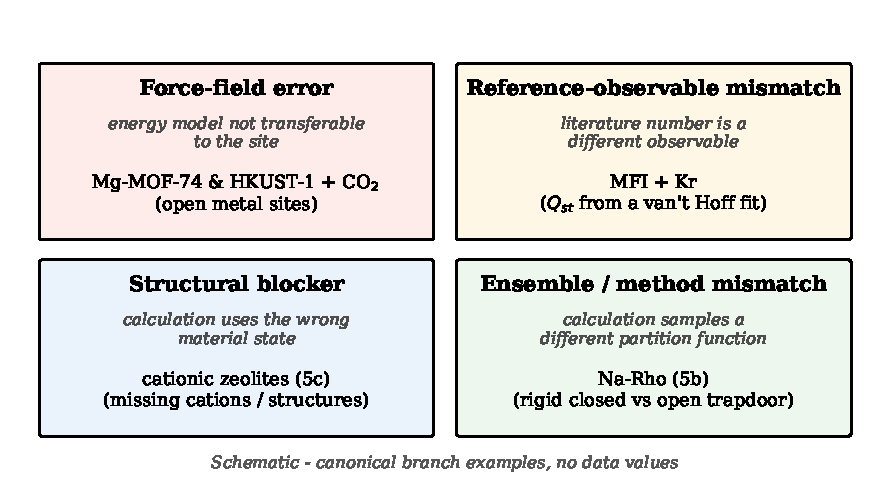
\includegraphics[width=0.86\textwidth]{figures/fig4_failure_taxonomy.pdf}
\caption{The four ways a calculated zero-coverage observable can lose contact with experiment, each with its canonical v0.4 branch example: force-field error (Mg-MOF-74 and HKUST-1 + CO\(_2\)), reference-observable mismatch (MFI + Kr, whose \(Q_{st}\) reference is a van't Hoff fit), structural blocker (cationic zeolites, 5c), and ensemble/method mismatch (Na-Rho, 5b). This figure is schematic and carries no numerical data.}
\label{fig:taxonomy}
\end{figure}

\FloatBarrier

The open-metal-site systems give the clearest force-field lesson. Mg-MOF-74 + CO\(_2\) and HKUST-1 + CO\(_2\) contain strongly binding metal environments. In such sites, carbon dioxide does not merely see a generic Lennard-Jones wall. It probes electrostatics, induction, short-range repulsion, dispersion, and local coordination chemistry. A non-polarisable or simplified pairwise force field can be reproducible and still give the wrong adsorption thermodynamics. That is what the atlas records: not that Widom insertion broke, but that the chosen energy model is not transferable enough for the site.

The direction of the error also matters. Some open-metal-site branches over-bind, while simpler UFF-type baselines under-bind. These are not contradictions. They show that different approximate energy models fail in different ways. A fitted cross-pair can put too much attraction into the binding site. A generic baseline can miss the same site. Both can be wrong for physically meaningful reasons. The audit prevents either result from being mistaken for a general statement about the material itself.

One caveat sharpens these force-field lessons. The comparison here is between the locked recipe and \emph{experiment}, not between the recipe and the originating paper's own simulated value, so an apparent over- or under-binding could in principle reflect a recipe difference or under-sampling rather than the energy model itself. Where the source recipe can be reproduced from the locked inputs, the atlas does reproduce the source's own simulated energetics: for HKUST-1 the modified Cu--O(CO\(_2\)) potential reproduces the paddle-wheel site interaction energy to within about two kilojoules per mole, and for UiO-66 the simulated heat of adsorption falls inside the band reported by the same study. For those branches the disagreement with experiment is therefore a genuine force-field-transferability result. For several Mg-MOF-74 recipes, however, the originating papers do not report a comparable simulated Henry constant or zero-coverage heat in the locked evidence, and in one case the atlas heat differs substantially from the source's own simulated value. For those branches the attribution to an intrinsic force-field limitation is reported here as unresolved pending a source-paper parity calculation, rather than as a proven force-field flaw. The open-metal-site Henry constant is also dominated by rare deep-well insertions --- in a representative audit, the hundred strongest of five thousand insertions account for roughly ninety percent of the Henry constant --- so production-count sampling is required and a low-count estimate is not converged.

The zeolite branches teach a different lesson. The clean all-silica MFI + Ar and Si-CHA + CO\(_2\) passes show that the harness can work when the structure, force field, and reference are aligned. They do not prove that all zeolite adsorption recipes are reliable. MFI + CH\(_4\), MFI + Kr, and the older Si-CHA + CO\(_2\) recipe still miss the strict gate. In several of these cases the problem is not simply the Henry constant. The heat of adsorption is the more sensitive axis, and its literature reference may itself come from a fitted or indirect observable.

The UiO-66 result is useful precisely because it is not a strict pass. The explicit-hydrogen, Yang-charge branch 3b\_EHq lies inside the physical-accuracy band but outside the strict regression band. That is the correct classification for a material whose reported adsorption is sensitive to synthesis, defects, and reference extraction. Calling it a strict validation point would overstate the result. Calling it a complete failure would throw away useful physical agreement. Tier-B exists to avoid both errors.

The cationic-zeolite cases are not force-field failures yet. They are incomplete recipes. Extra-framework cations are part of the material, not optional decoration. A pure-silica topology cannot stand in for Na-ZK-5, Zeolite 5A, Zeolite 13X, or Zeolite 4A when carbon dioxide adsorption is controlled by cation sites. Until the cation positions, charges, force-field parameters, and framework composition are locked, the calculation is not defined well enough to judge. Recording these systems as reference-audited targets is therefore more honest than forcing a pass or fail.

Na-Rho is still more restrictive. Its scalar branch is method-blocked because the rigid closed-state calculation and the trapdoor adsorption experiment do not sample the same configuration space. The problem is not merely that the force field needs tuning. The measured adsorption involves a framework-opening process, while the scalar Widom calculation samples a closed framework. The site-geometry evidence can be audited separately, but the scalar Henry constant and heat comparison cannot be converted into an ordinary validation test without changing the method.

This is why the small pass count is not a weakness of the audit. It is the audit doing its job. A less conservative workflow could report a number for every branch and then hide the reasons for disagreement in a table of residuals. widom-atlas instead separates reproducible agreement from force-field transferability failure, reference mismatch, structural incompleteness, and ensemble mismatch. The result is less flattering, but more useful.

The practical consequence is clear. For screening or machine-learning workflows, an adsorption number should not be consumed without its recipe and verdict. A strict-pass branch can be used as a calibrated validation point. A Tier-B branch can support a weaker physical-accuracy claim. A force-field-disagreement branch warns that the score is not reliable for the chemistry being tested. A method-blocked branch says that a different simulation observable is needed. The output of the atlas is therefore not just \(K_H\) or \(Q_{st}\). It is the reason those numbers should or should not be trusted.
